\chapter{RESULTS AND DISCUSSION}
\section{Method of Measuring Accuracy of Approximated Coordinates}
There were three methods used in the measuring of the accuracy of the approximated latitude and longitude coordinates produced by the discussed methodologies in this study. These three are: 1) looking at the Mean Absolute Error of the approximated coordinates compared to the actual coordinates of the tweets in the dataset, 2) using the Haversine Formula to get the average distance of each approximated coordinate from its actual location, and 3) using the Vincety Formula in place of the Haversine Formula. It is to be noted that the LDA-LSA Double Filter (first methodology) used only half of the dataset as test data while the Dynamic Dictionaries Per Region method (second methodology) used the entire dataset. 

\subsection{Mean Absolute Error}
Python's Scikit-Learn library was used in measuring the Mean Absolute Error of the approximated coordinates versus the actual coordinates for both methodologies. The Mean Absolute Error value is a measure which determines the error of all the given values in a dataset relative to another set. The best possible result for a Mean Absolute Error score is 0 since this indicates that there is no disparity between any of the compared values.

The Mean Absolute Error scores for both methodologies are found in \ref{tab:acc_lit}.

\begin {table*}[h]
\centering
\caption {\textbf{Mean Absolute Error Scores of Methodologies}}
\label{tab:acc_lit} 
\begin{tabular}{ c  c  c  c }
\hline
Methodology	&Latitude  	&Longitude 	&Average \\
Type  &MAE   &MAE   &MAE   \\
   \hline

LDA-LSA  &1.66  &1.07  &1.36  \\
Dynamic Dicts. &2.02   &1.30   &1.66   \\  \hline
\end{tabular}
\end{table*}

\subsection{Haversine Formula}
The Haversine Formula is a trigonometric method of measuring the distance of two coordinates. This way of measurement assumes that the two points being measured against one another belongs in a spherical space. 

The results of applying the Haversine Formula to measure the distance of each approximated coordinate versus its actual coordinates are shown in Table 4.2.

\begin {table*}[h]
\centering
\caption {Haversine Formula Scores of Methodologies}
\label{tab:acc_lit2} 
\begin{tabular}{ c  c  }
\hline
Methodology	&Average Haversine   \\
Type  &Distance (in KM)     \\
   \hline

LDA-LSA  &223.94    \\
Dynamic Dicts. &271.71    \\  \hline
\end{tabular}
\end{table*}

\subsection{Vincenty Formula}
The Vincenty Formula functions in a similar way as the Haversine Formula. The only difference is that the Vincenty Formula is a more widely-used method of computation in GPS devices. In principle, the Vincenty Formula uses the same trigonometric principles of computing the distances between two coordinates in a spherical space.

The results of the Vincenty Formula on the two methodologies is shown in Table 4.3.

\begin {table*}[h]
\centering
\caption {Vincenty Formula Scores of Methodologies}
\label{tab:acc_lit3} 
\begin{tabular}{ c  c  }
\hline
Methodology	&Average Vincenty \\
Type  &Distance (in KM)   \\
   \hline

LDA-LSA  &223.15  \\
Dynamic Dicts. &270.75      \\  \hline
\end{tabular}
\end{table*}

\section{Visualization of Results}
This section tackles the visualization of the results of both methodologies. Geolocated tweets were grouped into clusters for the purpose of visualization. The geolocated tweets from the first methodology were clustered based on topics, while the tweets from the second methodology were clustered based on geographic region. 


\begin{figure}
    \centering
    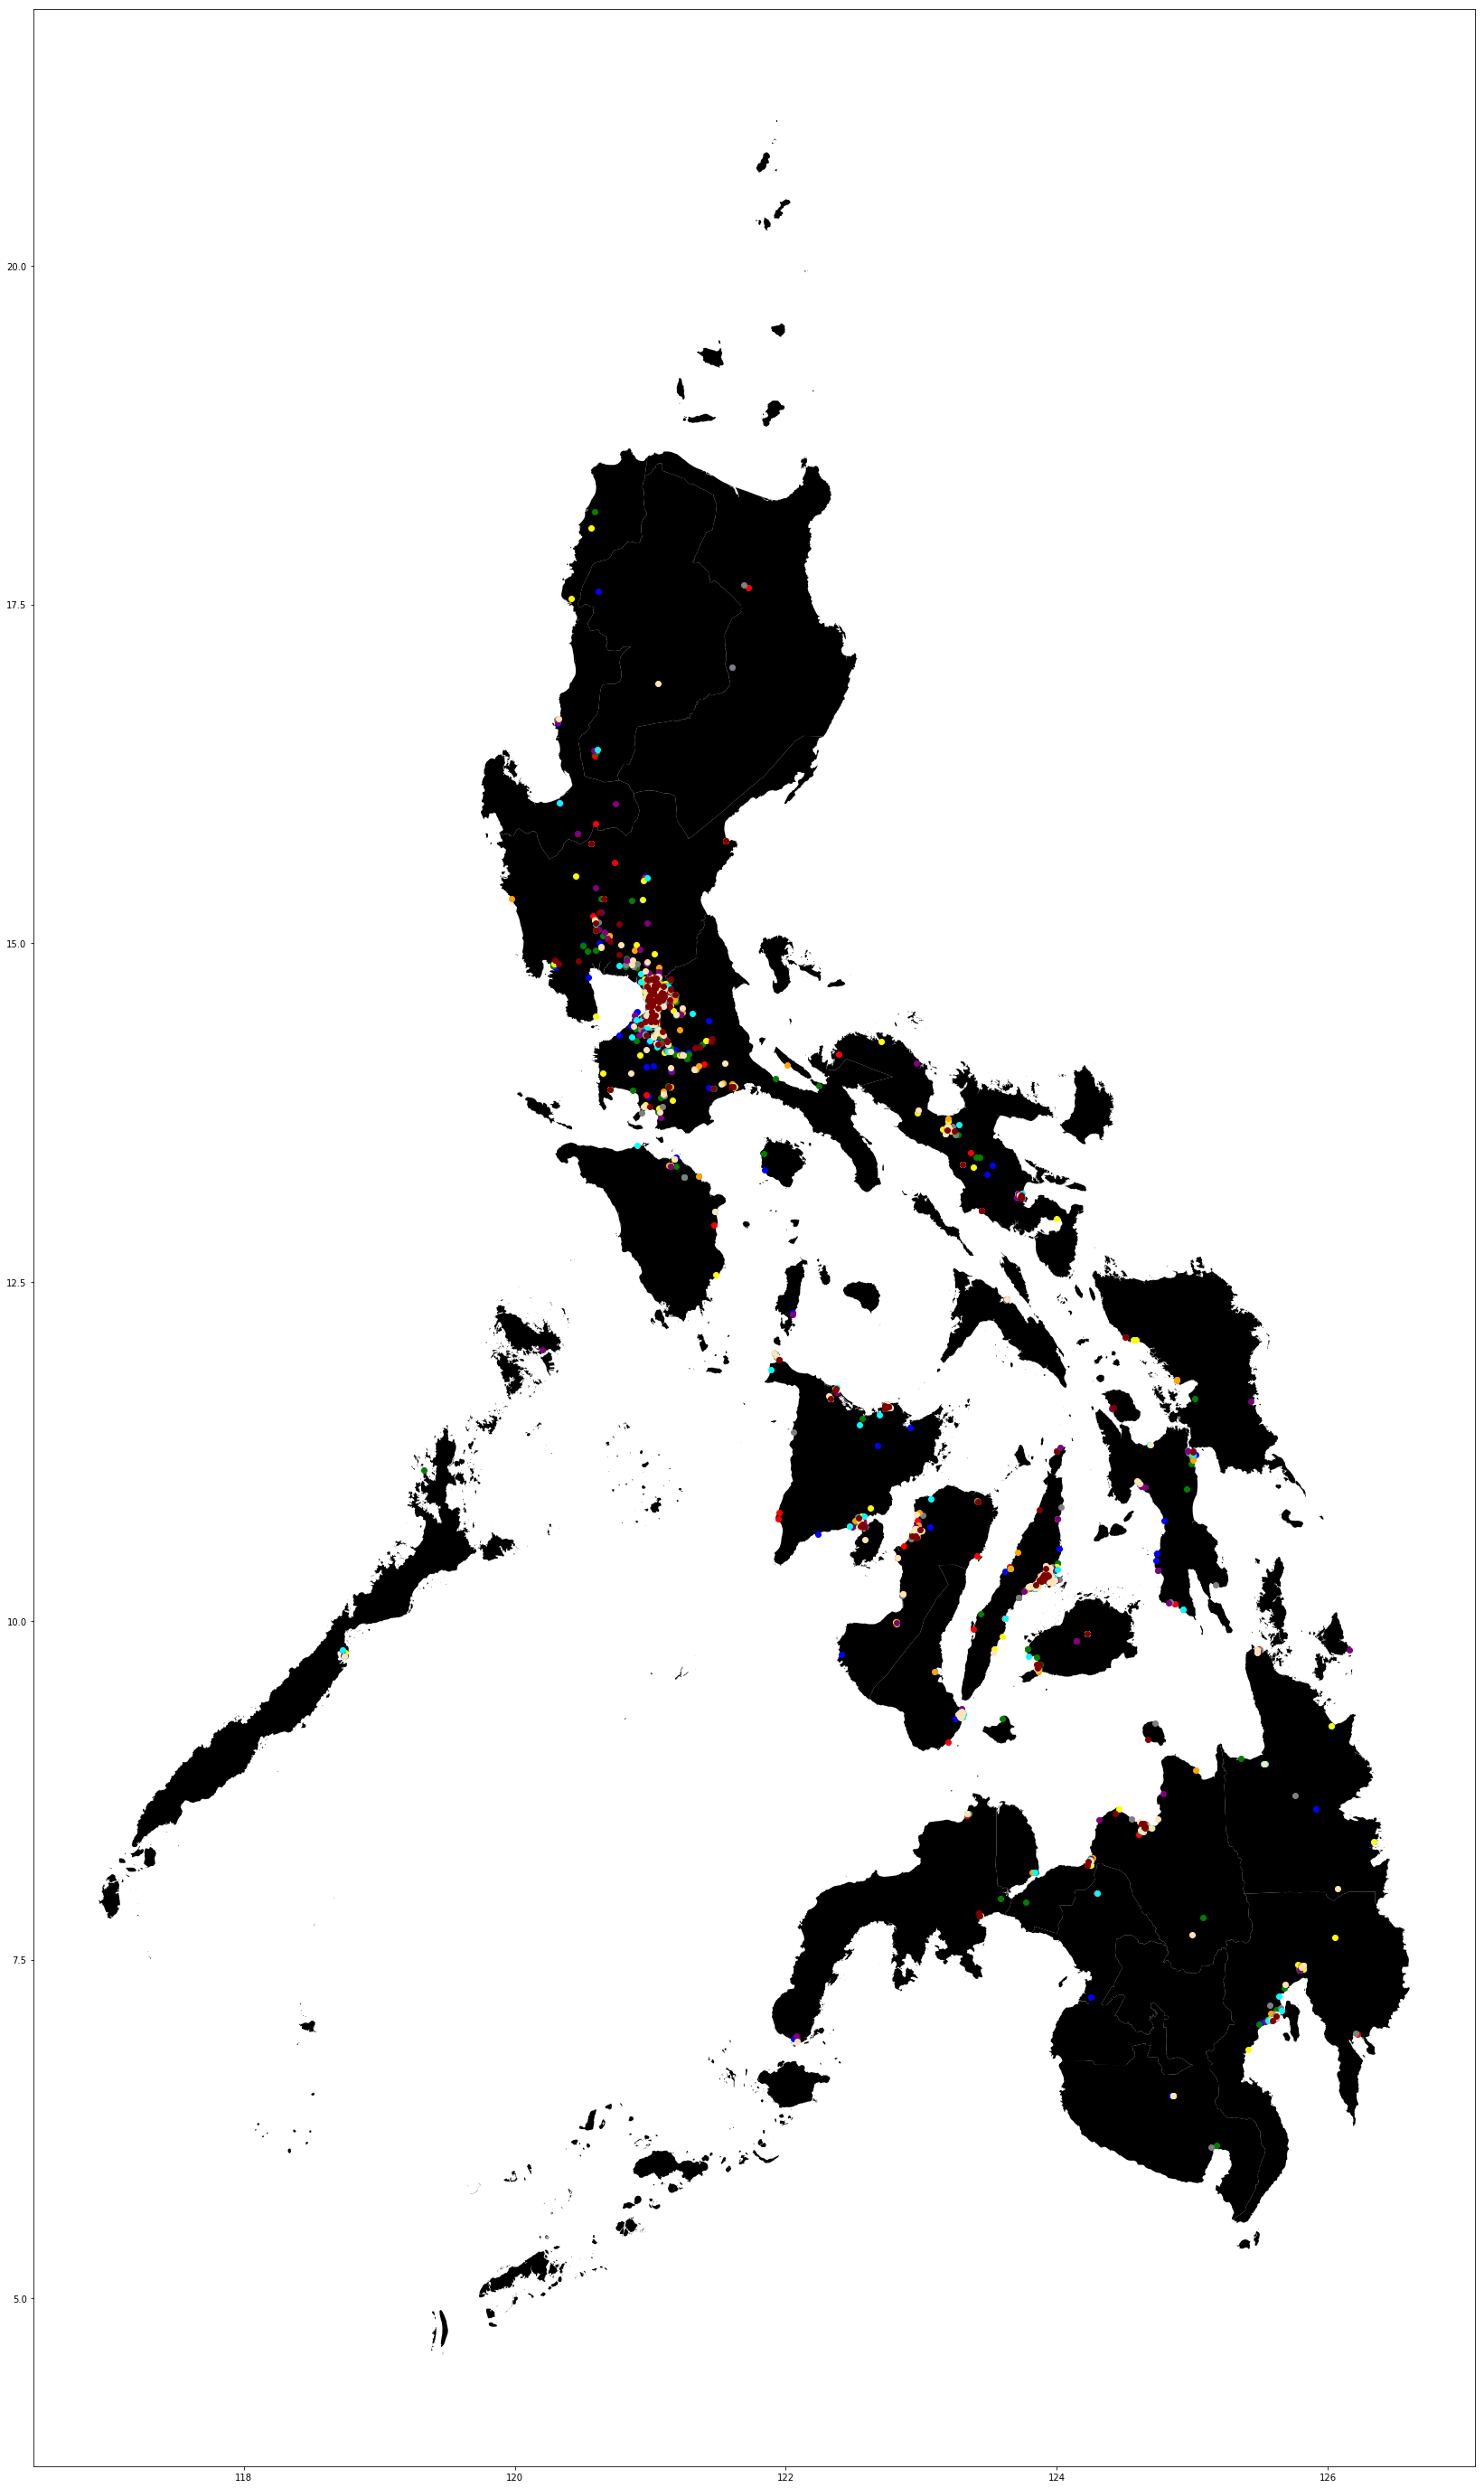
\includegraphics[width=\textwidth, height=\textheight,keepaspectratio]{Method1OrigMap.png}
    \caption{LDA-LSA Double Filter Plot of Original Tweets}
    \label{fig:my_label1}
\end{figure}

\begin{figure}
    \centering
    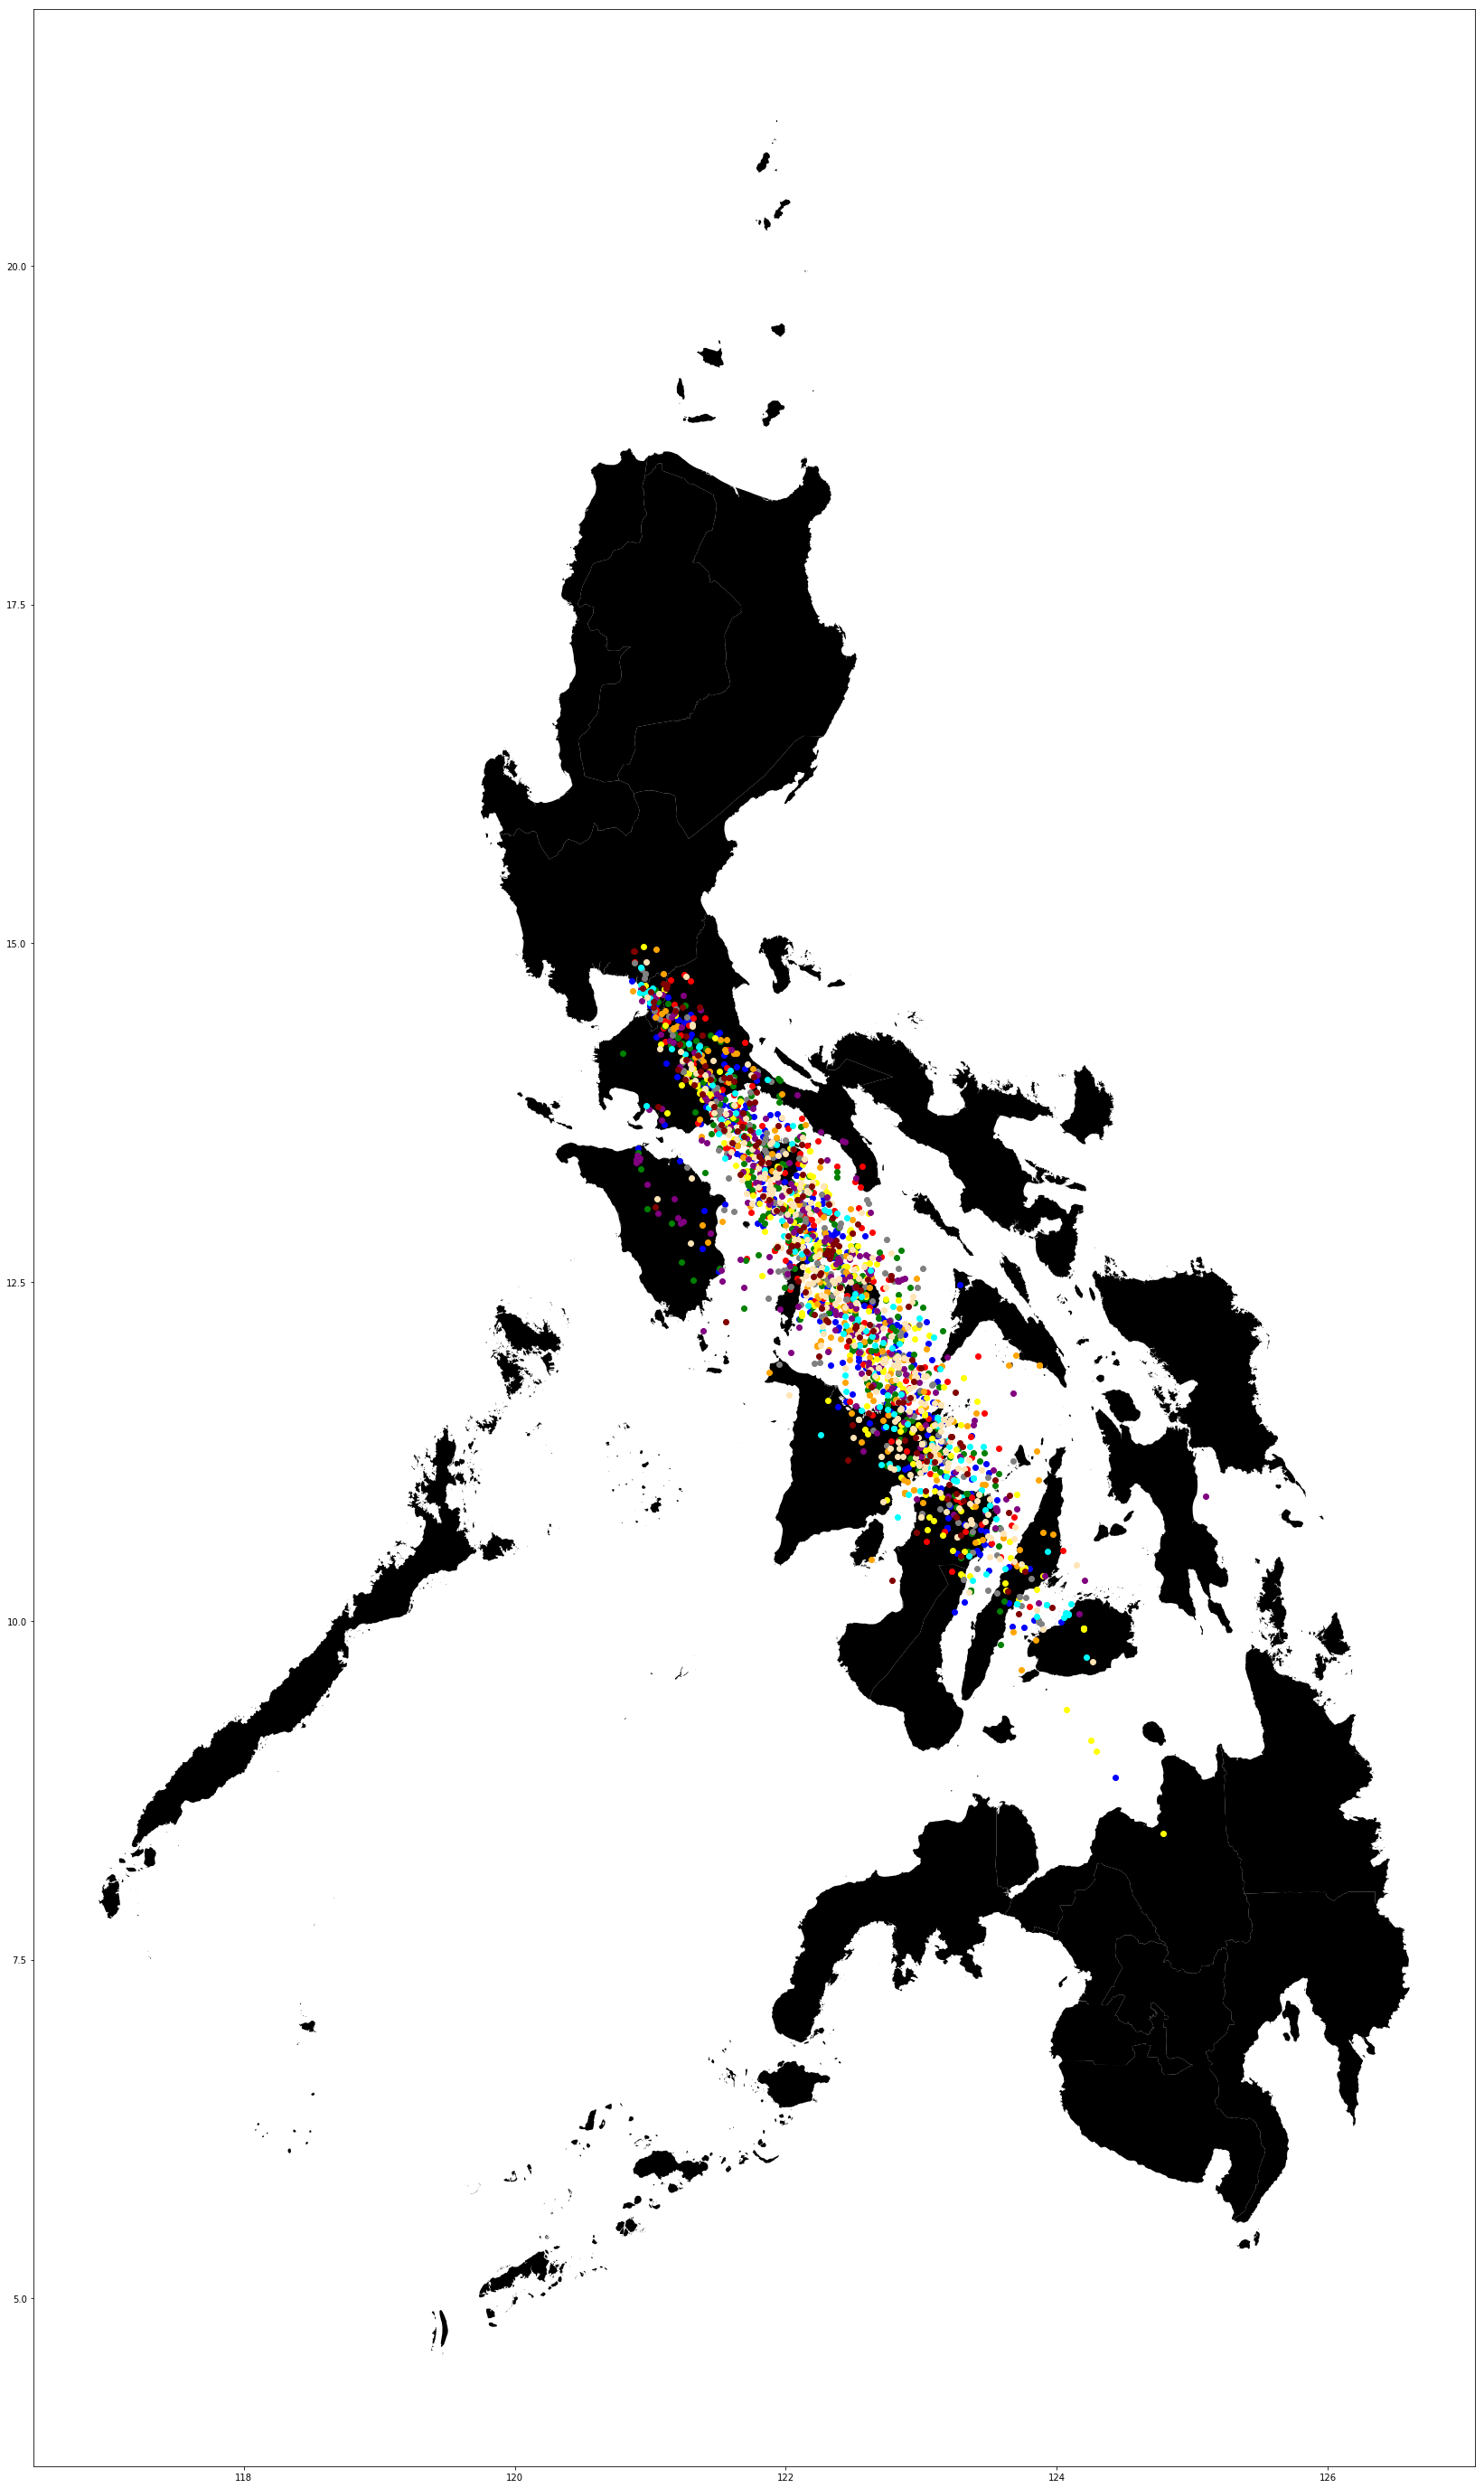
\includegraphics[width=\textwidth, height=\textheight,keepaspectratio]{Method1ApproxMap.png}
    \caption{LDA-LSA Double Filter Plot of Approximated Tweets}
    \label{fig:my_label2}
\end{figure}

\begin{figure}
    \centering
    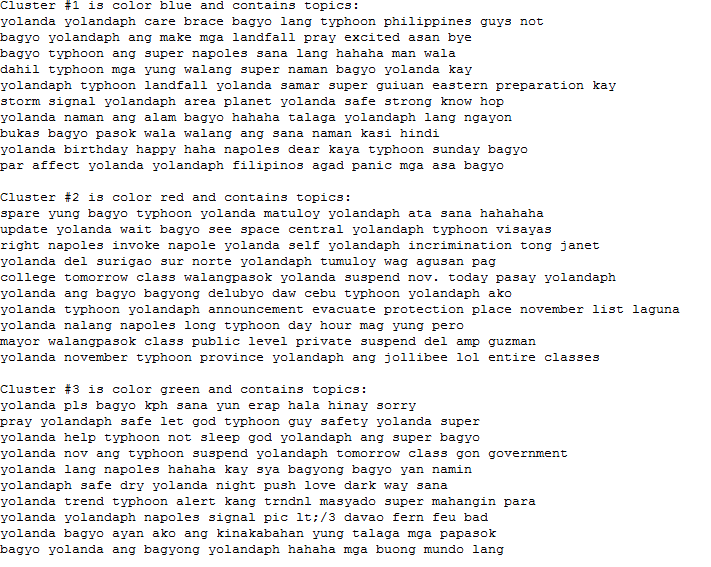
\includegraphics[width=\textwidth, height=\textheight,keepaspectratio]{Method1Cluster1.PNG}
    \caption{LDA-LSA Double Filter Clusters 1-3}
    \label{fig:my_label3}
\end{figure}


\begin{figure}
    \centering
    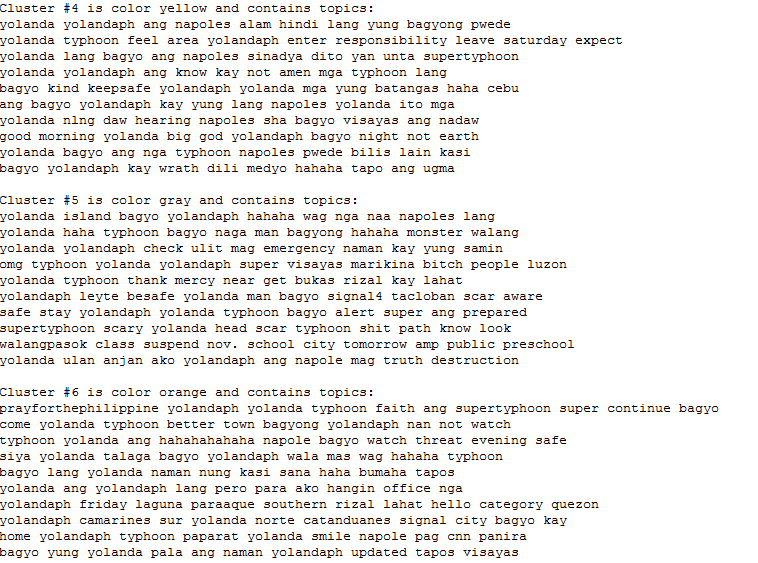
\includegraphics[width=\textwidth, height=\textheight,keepaspectratio]{Method1Cluster2.PNG}
    \caption{LDA-LSA Double Filter Clusters 4-6}
    \label{fig:my_label4}
\end{figure}

\begin{figure}
    \centering
    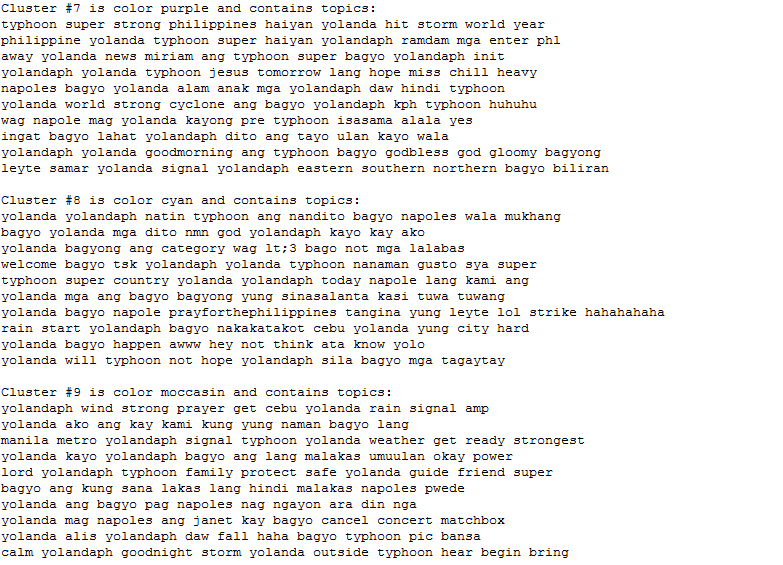
\includegraphics[width=\textwidth, height=\textheight,keepaspectratio]{Method1Cluster3.PNG}
    \caption{LDA-LSA Double Filter Clusters 7-9}
    \label{fig:my_label5}
\end{figure}

\begin{figure}
    \centering
    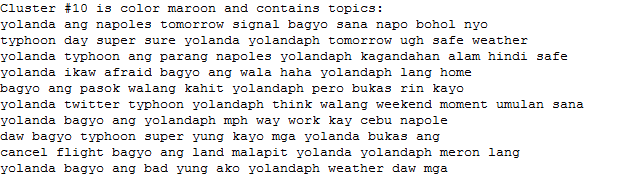
\includegraphics[width=\textwidth, height=\textheight,keepaspectratio]{Method1Cluster4.PNG}
    \caption{LDA-LSA Double Filter Cluster 10}
    \label{fig:my_label6}
\end{figure}

\begin{figure}
    \centering
    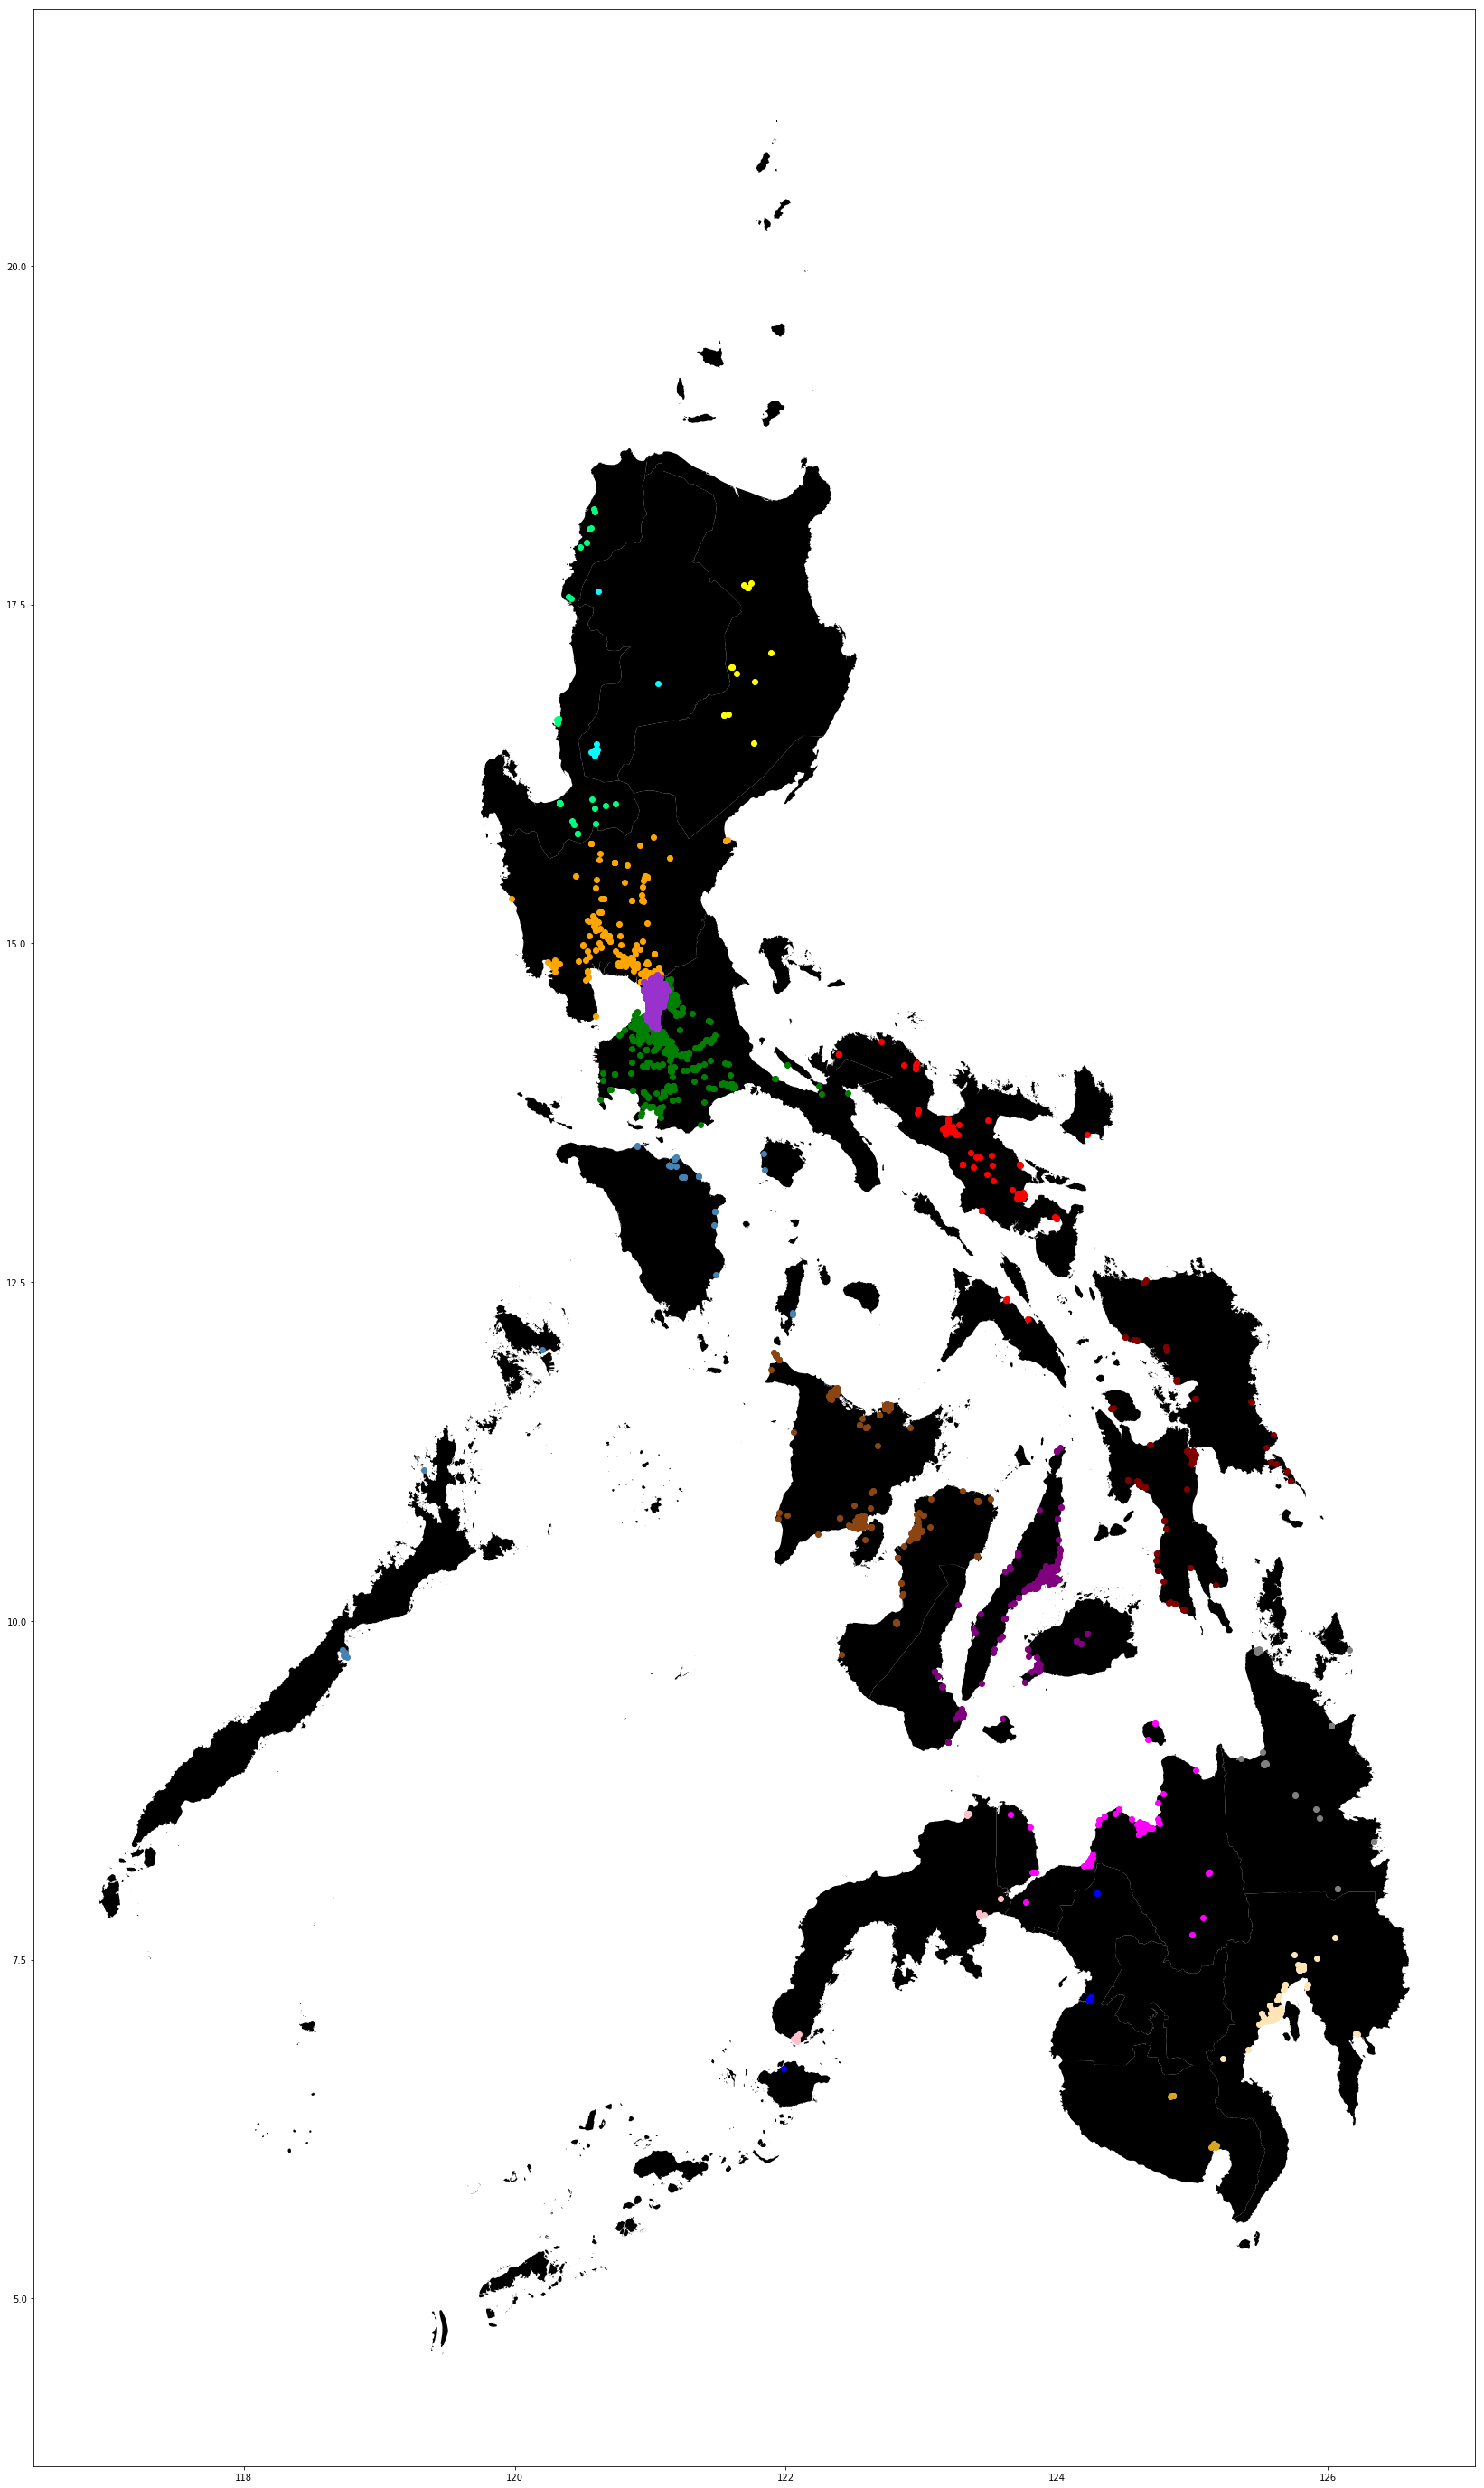
\includegraphics[width=\textwidth, height=\textheight,keepaspectratio]{Method2OrigMap.png}
    \caption{Dynamic Dictionaries Per Region Plot of Original Tweets}
    \label{fig:my_label7}
\end{figure}

\begin{figure}
    \centering
    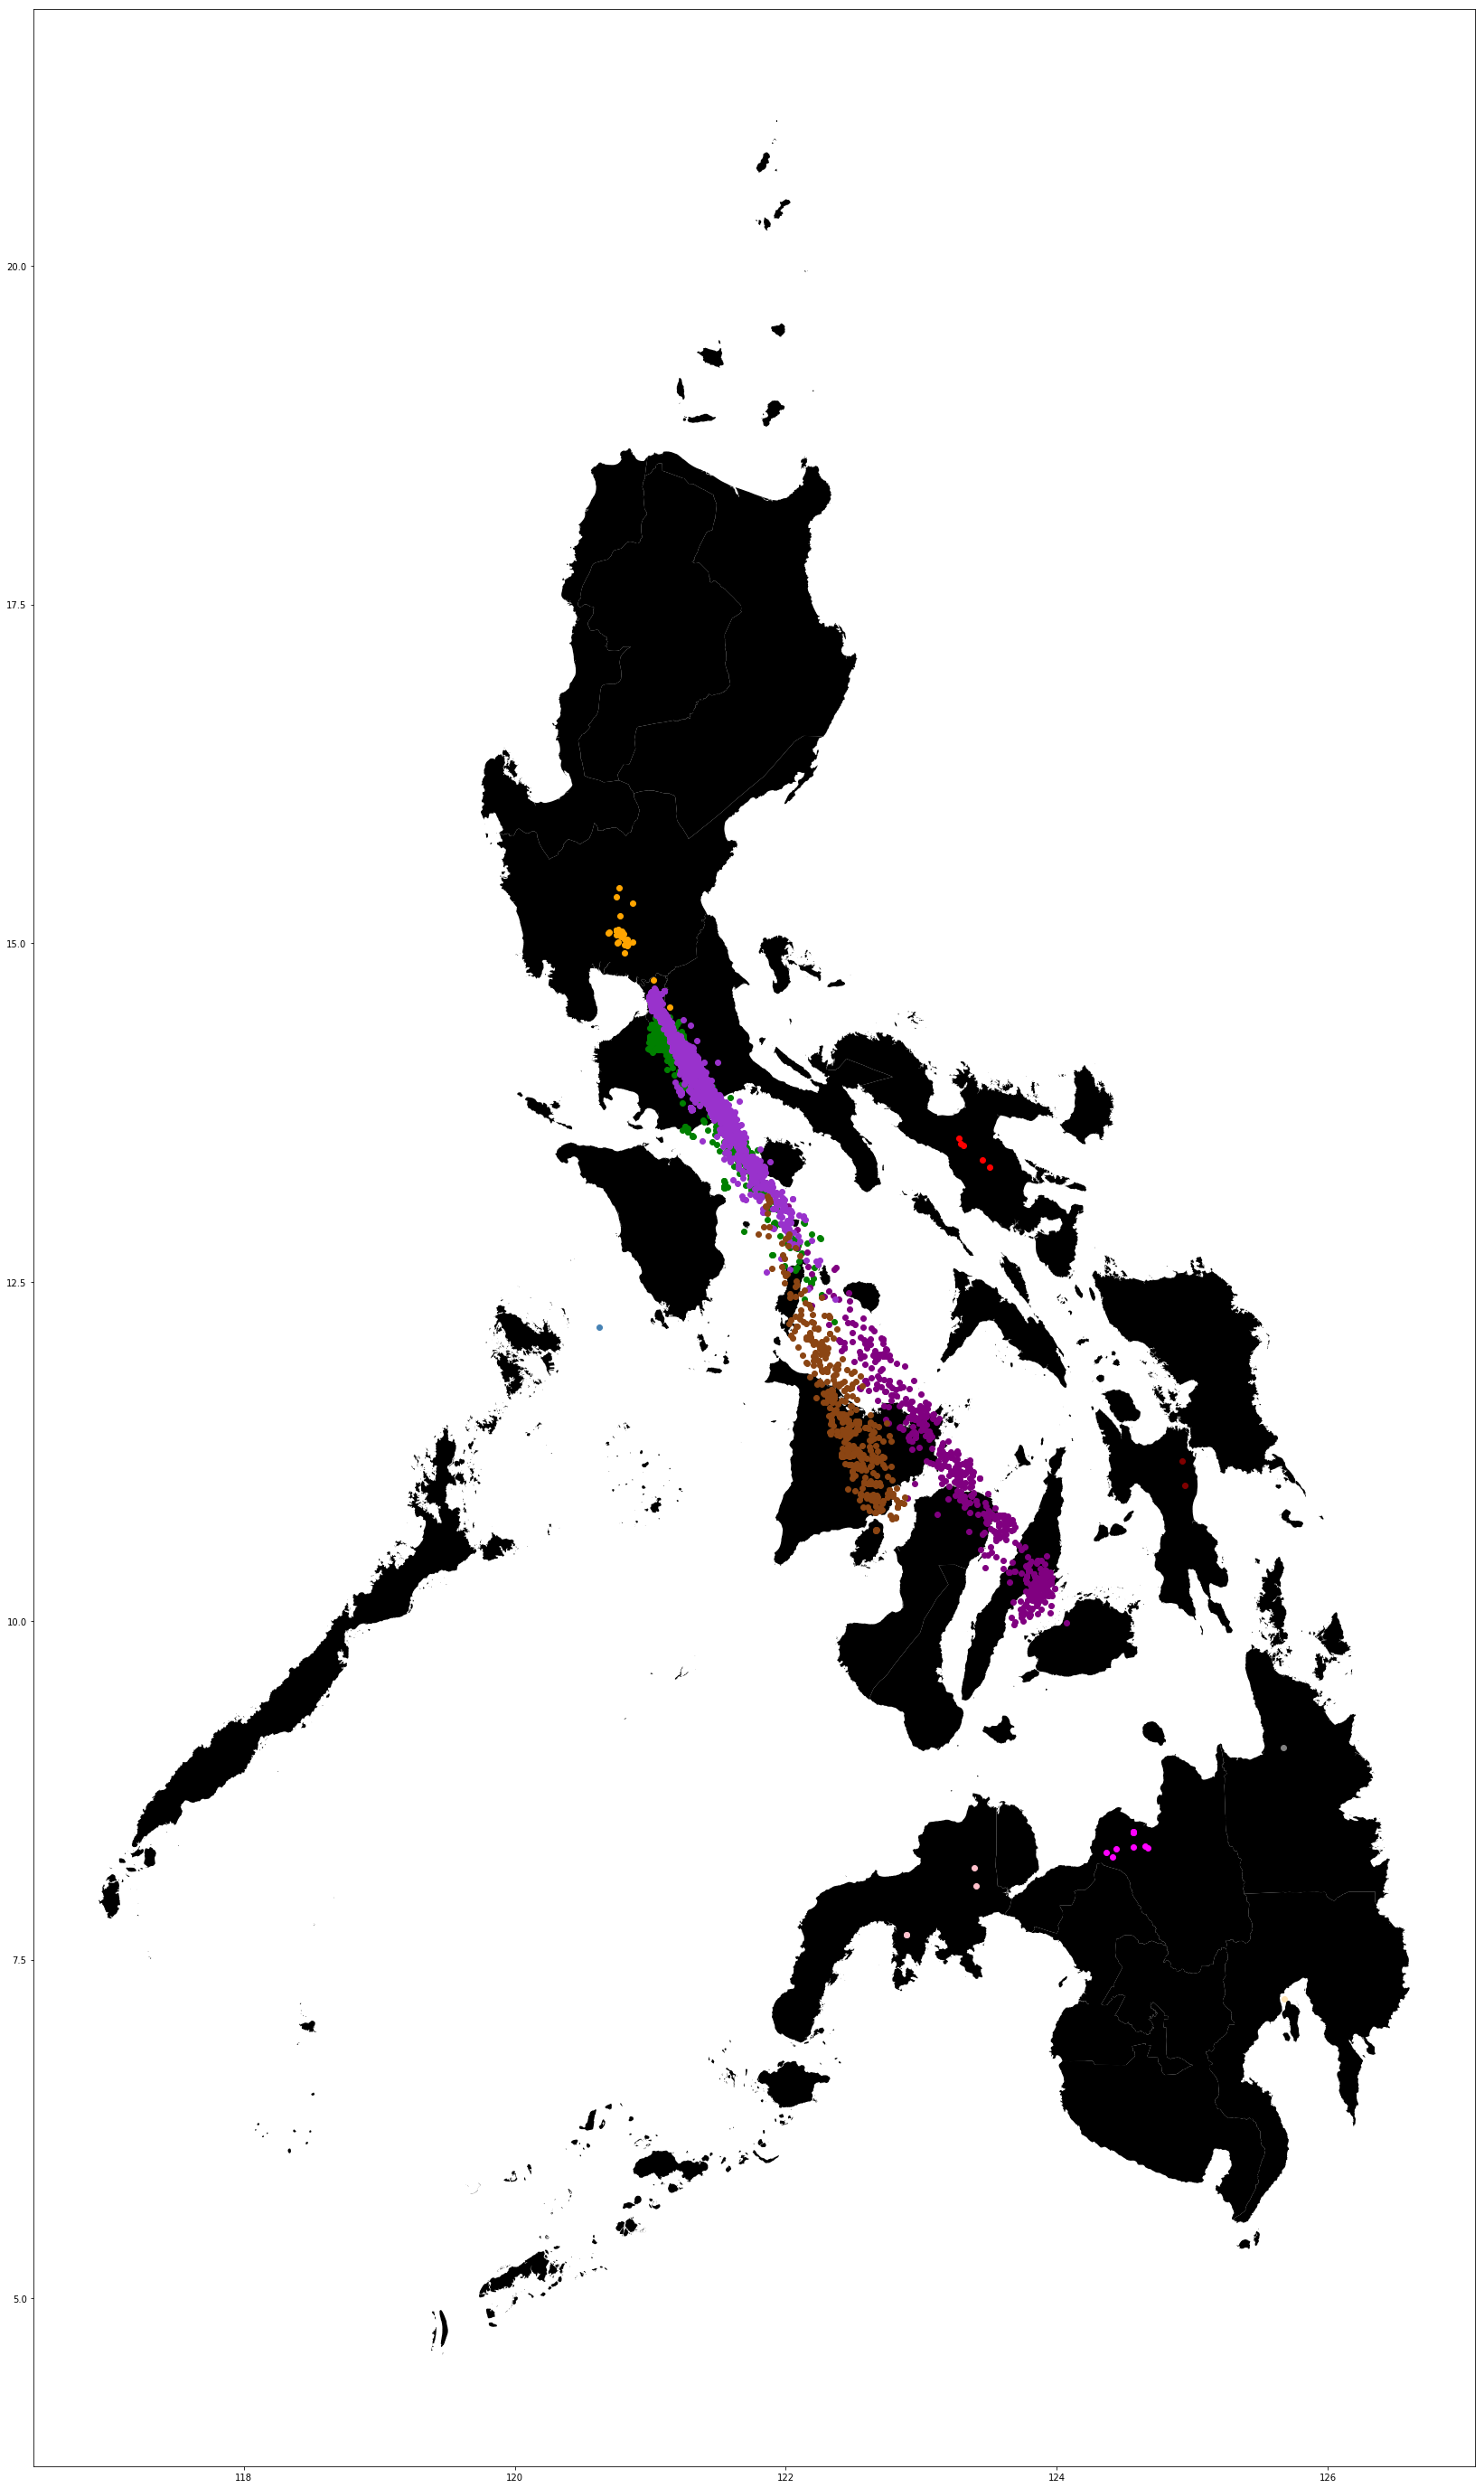
\includegraphics[width=\textwidth, height=\textheight,keepaspectratio]{Method2ApproxMap.png}
    \caption{Dynamic Dictionaries Per Region Plot of Approximated Tweets}
    \label{fig:my_label8}
\end{figure}

\begin{figure}
    \centering
    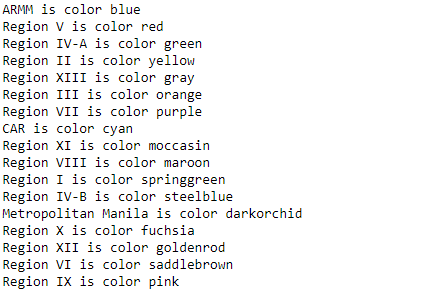
\includegraphics[width=\textwidth, height=\textheight,keepaspectratio]{Method2Cluster.PNG}
    \caption{Dynamic Dictionaries Per Region Clusters}
    \label{fig:my_label9}
\end{figure}

\subsection{LDA-LSA Double Filter Visualized Results}
Figure \ref{fig:my_label1} to \ref{fig:my_label6} shows the plots and cluster legend for the results of the first methodology. Figure \ref{fig:my_label1} shows that the original tweets that were clustered into the same topics were not necessarily within close geographic proximity among each other. In the case of some clusters, there were tweets that belonged in different parts of the Philippines. For example, there were tweets in Luzon and in Mindanao that were classified to the same cluster of topics. 

Figure \ref{fig:my_label2} shows the plot for the first methodology's geolocated tweets. As seen in the figure, the tweets belonging in the same cluster are more geographically clumped up together in general. It may be noted that the majority of the tweets were approximated to be located near the Visayas region and south of the NCR. It is also apparent that there are groups of tweets that were geolocated in invalid locations such as bodies of water. 

Figures \ref{fig:my_label3} to \ref{fig:my_label6} serve as the legend of clusters for Figures \ref{fig:my_label1} and \ref{fig:my_label2}. There were ten clusters used for the LDA-LSA Double Filter methodology. Each cluster contains ten topics in string form with similar themes. The ten clusters used reflect the number of topics that were used to train the LDA model as discussed in the methodology section. The color for each cluster of topics are also specified. 

\subsection{Dynamic Dictionaries Per Region Visualized Results}
Figures \ref{fig:my_label7} to \ref{fig:my_label9} display the plots and cluster legend for the Dynamic Dictionaries Per Region methodology. Figure \ref{fig:my_label7} contains the plot of the original tweets from the dataset used in this study. It may be observed that all Philippine geographic regions contain at least one tweet in their vicinity, with a majority of them being located in Central Luzon. 

Figure \ref{fig:my_label8} is the plot of the geolocated tweets from the Dynamic Dictionaries Per Region methodology algorithm. There are some Philippine geographic regions shown in Figure \ref{fig:my_label8} that do not contain any tweets unlike in Figure \ref{fig:my_label7}. It is also worth noting that there were groups of tweets that were geolocated in bodies of water similar to the case of the LDA-LSA Double Filter methodology. Lastly, Figure \ref{fig:my_label9} shows the legend of clusters for the Dynamic Dictionaries Per Region methdology.

All plots and figures were created via Python scripts. Any program that has Python support may recreate these plots accordingly. 

\section{Insights}
The results of both methodologies provide several insights. It appears that the first methodology (LDA-LSA Double Filter) outperformed the second (Dynamic Dictionaries Per Region) in all three metrics used to measure the accuracy of the results of both.

The closer to zero the Mean Absolute Error of a dataset is compared to another, the better. Again, a value of 0 indicates that the values of a test dataset completely matches that of the values of a given target dataset. The Mean Absolute Error value of the first methodology is lower by 0.3 compared to the second. This means that the approximated coordinates from the first methodology are closer to the actual coordinates in the dataset than the ones from the second.

The Haversine Formula and Vincenty Formula results show a similar trend. The first methodology's scores are significantly better than the second's for both metrics. This indicates that the approximated coordinates from the first methodology are nearer to their actual coordinates from dataset in terms of kilometers. This means that given these results, it is more effective to approximate a given disaster-related tweet according to the topic it belongs to than its geographic region. 

A possible reason as to why the second methodology yielded worse results is because there are some Philippine regions that cover relative large geographic areas. This means that it is possible that the approximated latitude and longitude coordinates of a given tweet belongs in the same region as its original coordinates, but not necessarily in the same vicinity. Some areas within certain Philippine regions are separated by tens or even hundreds of kilometers. This may contribute to high distance disparity between the actual and approximated values. This is perhaps the main drawback of classifying tweets per region. 

Another possible reason as to why the first methodology outperformed the second is the structure of the dataset that was used in this study. It was found that over sixty percent of the tweets in the dataset belonged in the NCR and that some regions contained anywhere from nine to twenty-five tweets only. This may cause the execution of the second methodology to perform worse because the models representative of all geographic regions are not equally refined/trained. There are some models that are more refined than others since the number of tweets are not equally distributed across all available regions. This conversely means that some models are poorly trained because there are only several tweets from that region as far as the dataset used is concerned. The differences in refinement of the geographic models may cause the models to classify a given query tweet to the incorrect region because it is more likely that the more refined models will be selected by the algorithm described in the previous sections. The richer models have more depth in terms of stored information and thus are more capable of processing and identifying incoming query tweets as part of the geographic region they represent. It is highly likely that there are many cases where, for example, a tweet originally from the ARMM region may be recognized and classified as a tweet from the NCR since the model representative of the latter region is much better trained. This kind of scenario becomes increasingly likely to happen as the algorithm executes because the models refresh periodically after processing a certain number of tweets. The better trained models will be continuously further trained and refined as they process more tweets.

These results however do not discount the fact that both methodologies still performed better than previous studies did as far as the Typhoon Yolanda tweets are concerned. An over 200 kilometer distance is still large, but this is a significant improvement from the findings of the previous studies discussed in the theoretical background section of this paper. The said previous studies had results of over 300 kilometers of distance for the approximated coordinates. Both methodologies had below 300 kilometers, which is a slight improvement. But again, the results indicate that while both methodologies are possible steps towards the right direction, the first methodology appears to be the more optimal approach for this dataset. It is also worth noting that the results of both methodologies showed that there were still quite a number of tweets that were geolocated in invalid locations such as bodies of water. Again, this is reflective of the fact that the Philippines is an archipelago, and that both methodologies may still be improved tremendously. 